\chapter{Zahlenfolgen, Zahlenreihen, Konvergenz}

Der moderne Grenzwertbegriff stellt die Grundlage der Infinitesimalrechnung dar. In diesem Kapitel betrachten wir zuerst Zahlenfolgen und Reihen, definieren dann Konvergenz sowie Grenzwert und lernen abschließend
einige wichtige Regeln zur Konvergenz und Grenzwertbestimmung kennen.

Um die Wichtigkeit zu illustrieren, warum eine exakte Definition der Konvergenz notwendig, sei Zenons Paradoxon von Achilles und der Schildkröte angeführt. \emph{Zeno of Elea} (etwa 500 BC) hat dieses Paradoxon angeführt, um zu zeigen, dass der naive Begriff von Wandel und Bewegung nur eine Illusion wäre. Zur besseren Veranschaulichung wählen für die folgende Erklärung (willkürlich gewählte) Größenabgaben. In dem Paradox nun veranstalten Achilles und eine Schildkröte ein Wettrennen, wie in Abbildung \ref{fig:ZenoAchilles} dargestellt. Achilles ist in der Lage, mit einer Geschwindigkeit von $25\ukmh$ zu rennen, während die Schildkröte nur $5\ukmh$ schafft. Der Fairness halber erhält die Schildkröte daher einen Vorsprung von $100\ukm$. Die Frage ist nun, wann Achilles die Schildkröte überholt. Der geläufige physikalische Ansatz wäre, ein Koordinatensystem zu definieren, die Bewegungsgleichungen beider Partizipanten aufzustellen und den Schnittpunkt zu berechnen. Zenon argumentiert allerdings wie folgt:

\begin{enumerate}
	\item Damit Achilles die Schildkröte überholen kann, muss er zunächst den Vorsprung von $100\ukm$ aufholen. Dazu benötigt er $4$ Stunden.
	\item In diesen $4$ Stunden allerdings ist die Schildkröte bereits $20\ukm$ weiter gekrochen.
	\item Also muss Achillles im nächsten Schritt diese $20\ukm$ Vorsprung aufholen, wozu er $0.8$ Stunden benötigt. Aber nun hat die Schildkröte bereits einen neuen Vorsprung erhalten.
	\item Egal, wie oft Achilles also den Vorsprung aufholt, um die Schildkröte zu überholen, müsste er unendliche viele Vorsprünge aufholen. Also holt Achilles die Schildkröte nie ein, um kann sie somit auch nicht überholen.
\end{enumerate}

Wie lässt sich dieses Paradoxon auflösen? Der Fehler, den Zenon hier begeht, besteht darin, dass Achilles zum Aufholen "unendlicher" vieler Vorsprünge auch "unendlich" viel Zeit benötigt. Dies ist aber bei einer genauen Betrachtung mithilfe eines exakten Grenzwertbegriffs nicht der Fall, wie wir auch in einer Übungsaufgabe nachweisen werden.

\begin{figure}[H]
	\caption{Zenos Paradoxon von dem Wettrennen zwischen Achilles und der Schildkröte}
	\label{fig:ZenoAchilles}
	\centering
	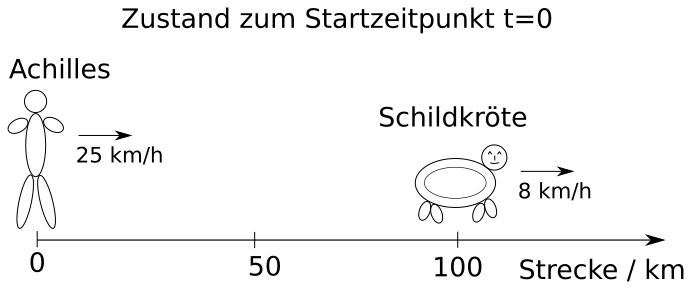
\includegraphics[width=0.95\textwidth]{./svg/zeno-achilles.png}
\end{figure}



\section{Zahlenfolgen und Reihen}

Bevor wir den Begriff der Konvergenz näher definieren können, benötigen wir zuerst ein Verständnis von Zahlenfolgen.

\begin{definition}[Unendliche Zahlenfolge]
	Eine unendliche Zahlenfolge ist gegeben, wenn jeder natürlichen Zahl $n \ge 0$  genau eine (meist reelle) Zahl $a_n\in\R$ zugeordnet wird. $a_n$ heißt das $(n+1)$-te Glied der Zahlenfolge.
\end{definition}

\begin{definition}[Endliche Zahlenfolge]
	Besteht die Zuordnung nur für jede natürliche Zahl $n$ zwischen 0 und $N$ ($0 \ge n \ge N$), so spricht man von einer endlichen Folgen.
\end{definition}

Zahlenfolgen können also als Funktion $f: \N \to \R$ aufgefasst werden. Zur mathematischen Darstellung gibt es zwei Möglichkeiten:

\begin{enumerate}
	\item Explizite Darstellung: Der Wert des $n$.-ten Folgenglieds ist direkt gegeben. 
	\item Implizite (rekursive) Darstellung: Der Wert des nächsten Folgengliedes ($n+1$) ist gegeben in Abhängigkeit eines oder mehrerer voriger Folgenglieder. Zudem ist ein Startwert für das erste oder die ersten Folgenglieder gegeben.
\end{enumerate}

Wir wollen uns diese beiden Möglichkeiten an zwei wichtigen Zahlenfolgen anschauen.

\begin{definition}[Arithmetische Zahlenfolge]
	Eine arithmetische Zahlenfolge ist gegeben, wenn in jedem Schritt das nächste Folgenglied durch Addition einer Konstanten zum vorigen Folgenglied bestimmt wird.
\end{definition}

\begin{definition}[Geometrische Zahlenfolge]
	Eine geometrische Zahlenfolge ist gegeben, wenn in jedem Schritt das nächste Folgenglied durch Multiplikation einer Konstanten mit dem vorigen Folgenglied bestimmt wird.
\end{definition}

Eine arithmetische Zahlenfolge beschreibt konstantes Wachstum und kann auch als lineare Funktion aufgefasst werden. Demgegenüber drückt eine geometrische Zahlenfolge exponentielles Wachstum, etwa die (initiale) Vermehrung von Bakterien in einer Petrischale. In \ref{lst:ExArithGeo} sind diese beiden Zahlenfolgen anhand eines konkreten Beispiels in beiden Darstellungsformen zu sehen

\begin{listing}[h]
	\label{lst:ExArithGeo}
	\caption{Beispiel für arithmetische und geometrische Zahlenfolge}
	Die arithmetische Zahlenfolge der ungeraden Zahlen beginnt mit $(a_n) = 1, 3, 5, 7, 9, ...$. Das Zahlenfolgenglied für $n=0$ ist $a_0=1$. Für $n=1$ ist $a_1=3$, für $n=2$ ist $a_2=5$. Wir erkennen sofort,
	dass ein Folgenglied immer um $2$ größer ist als das vorige. Die rekursive Darstellung lautet somit also $a_{n+1} = a_n + 2$ mit dem Startwert $a_0 = 1$.  Wenn wir es nun noch schaffen, eine Formel für $a_n$ in Abhängigkeit von $n$ zu finden, haben wir auch die explizite Darstellung gefunden: $a_n = 2n+1$.
	
	Analoges gilt für die geometrische Zahlenfolgen. Beispielsweise ist $(a_n) = 1, \frac{1}{2}, \frac{1}{4}, \frac{1}{8}, \frac{1}{16}, ...$ eine geometrische Zahlenfolge. Jedes Folgenglied ergibt sich, indem das
	vorige Folgenglied halbiert wird. Damit können wir die rekursive Darstellung angeben als $a_{n+1} = \frac{1}{2}a_n$ mit dem Startwert $a_0=1$. Für die explizite Darstellung erhalten wir nach etwas Nachdenken $a_n = {\frac{1}{2}}^n$. Wichtig zu betonen ist hier, dass es keine allgemein gültige Vorgehensweise gibt, die rekursive Darstellung in die explizite Darstellung umzuwandeln, hier ist wie in vielen Teilen der Mathematik kreatives Nachdenken erforderlich.
\end{listing}



\section{Konvergenz und Grenzwertbegriff}

\section{Konvergenzanalyse}

\section{Grenzwertregeln}
